\chapter{Defeasible Reasoning}
\label{chapter:defeasible-reasoning}

Non-monotonicity in logical systems has been the focus of study for decades, and several distinct formalisms have been developed.
The motivation is to expand the inference power beyond that of the classical, to a more credulous one where inferences may,
upon learning new information, be retracted.

This work is interested in the kind of non-monotonic reasoning put forward by Kraus, Lehmann, and Magidor \cite{kraus1990nonmonotonic,lehmann1992what},
frequently initialised to the \textit{KLM framework}.

\textcolor{red}{This could be a bit more discursive I think}

\section{Background on Non-monotonic Reasoning}
\label{section:nmr-background}

Near the end of the previous chapter, the matter of consequence was discussed in a very formal sense. It is perhaps
helpful to distinguish this subject---classical consequence---from the common concept, as the former yields some surprising
results which do not appear at all congruent with how a person, or otherwise intelligent agent should reason
\cite{tarski1936consequence, kraus1990nonmonotonic}. As a demonstration of a result which may be surprising in this way,
consider the following propositions, which state that \textit{humans experience chronological time \text{,} soldiers are
human}, and \textit{Billy Pilgrim experiences non-chronological time}.
\begin{enumerate}
	\item $\texttt{human}\rightarrow \texttt{chronological time}$

	\item $\texttt{soldier}\rightarrow \texttt{human}$

	\item $\texttt{Billy Pilgrim}\rightarrow \neg \texttt{chronological time}$
\end{enumerate}

Knowing these propositions, if we were to encounter an individual in combat fatigues we might find it sensible---by propositions
2 and 1---to deduce that the individual experienced time chronologically. If we were to later learn that the individual
were, in fact, Billy Pilgrim, given proposition 3, we should like to retract our prior inference and replace it with the
knowledge that the individual does not experience time chronologically.

Such recourse is not, as it stands, possible. When we see the that the individual is a soldier, the possible worlds
satisfying our existing knowledge are reduced to the single model: $\{\overline{b},c,h,s\}$ (where $b$: \texttt{Billy
Pilgrim}, $c$: \texttt{chronological time}, $h$: \texttt{human}, and $s$: \texttt{soldier}). Should we later learn that the
individual is indeed Billy Pilgrim, the theory becomes inconsistent.
%TODO: Add section in preliminaries about principle of explosion
And, by the principle of explosion, discussed in \Cref{subsection:logical-consequence}, our theory now entails that the
individual experiences time both chronologically and non-chronologically. Indeed, our theory now entails everything and
is accordingly worthless.

This property of classical logic---that adding new information never results in retraction of pre-existing knowledge---is
called monotonicity. The presence of monotonicity requires that when we make a claim such as \say{humans experience time chronologically},
we must be absolutely sure of ourselves, so as to never worry about needing to retract an inference. This is, of course,
too strict a requirement as we cannot determine for all future, present, and past humans if it were the case that they experienced
time chronologically. If we remain in the classical realm, it seems our only options are to abandon our original claim or
risk explosion.

At this point it is a good idea to provide some clarification on how we might begin to approach solutions to this issue.
Continuing with the same example---and continuing to allow ourselves to entertain the possibility of experiencing non-chronological
time---it would certainly be agreed that typically soldiers are human, and also that typically humans experience time chronologically.
To resolve that Billy Pilgrim is a soldier, and therefore a human, who does not experience chronological time, we need only
to point out that he may be an atypical human, and so the qualities we associate with typical humans need not apply to
him.

To make the previous paragraph more formal, we remind the reader of the discussion held around \Cref{definition:logical-consequence}:
A formula $\phi$ is a logical consequence of a set $\Gamma$ thereof if every model of $\Gamma$ is also a model of $\phi$.
Put differently, there is no valuation (or, possible world) where $\Gamma$ is true and $\phi$ is false. It follows
directly that $\phi$ remains a logical consequence of $\Gamma \cup \{\psi\}$, since $\Gamma$ is true in any world where $\Gamma
\cup \{\psi\}$ is true. It was pointed out by Shoham \cite{shohamSemanticApproach} that we may \say{bend the rules} and restrict
semantic consideration to a privileged subset of models deemed ``preferable''. We call these selected models the \textit{minimal
models}---the reasons for this name should become clearer as the chapter progresses.

\section{The KLM Framework}
The KLM framework for non-monotonic reasoning was initially described by a collection of consequence relations satisfying
certain axioms---frequently called the \textit{rationality postulates}. We borrow a nice story from Dov Gabbay \cite{gabbay1985theoreticalFoundations}
which motivates why consequence relations are a good starting point for the study of non-monotonic systems.

Paraphrasing, he begins by asking the reader to imagine a machine that does non-monotonic inference in some domain. The machine
represents knowledge as formulae and so we pose queries of the form \say{Does $\psi$ non-monotonically follow from $\phi$?}.
Something goes awry (suppose some coffee was spilled), calling into question whether the logic of the machine still
functions correctly. Even worse, the interface, which tells us what real-world instance each formula maps to, is
destroyed and so function cannot be evaluated based on the meaning of the formulae the machine reasons on. How might we then
evaluate the machine's function?

If we were interested in classical consequence, we would be well-equipped to assess the correctness of the machine by
determining if it satisfied reflexivity, monotonicity, and cut (we point to \Cref{definition:consequence-relations} as a
reminder). This is precisely the starting point that Kraus, Lehmann, and Magidor took up in \cite{kraus1990nonmonotonic},
suggesting that before getting to the semantics of a non-monotonic system, it is a good idea to formalise axiomatise the
system as a consequence relation satisfying certain properties.

The rationality postulates are precisely this axiomatisation, characterising a sensible pattern of reasoning for non-monotonic
systems. We use `$\twiddle$' (pronounced ``twiddle'') instead of `$\vdash$' to denote a non-monotonic consequence relation.
As we may expect, $\phi \twiddle \psi$ has the same meaning as $(\phi, \psi) \in \; \twiddle$, and $\phi \ntwiddle \psi$
as $(\phi, \psi)\not \in \; \twiddle$. We may, at times of potential confusion, use a subscript to disambiguate which consequence
relation is being referred to, and so $\twiddle_{C}$ would refer to a cumulative relation, as defined below.

\subsection{Cumulative Reasoning}
\label{subsection:system-c} \index{non-monotonic reasoning! system C}

\textit{Cumulative consequence relations}, otherwise referred to as \textit{System C}, represent the weakest of the
systems in the KLM framework. We follow the same exposition, from weaker to stronger systems, as \cite{kraus1990nonmonotonic}:
this approach will minimise repetition, as each successive system inherits all properties of its predecessor.

\begin{definition}
	\label{definition:cumulative-consequence-relation} \index{consequence relations! cumulative}

	A consequence relation $\twiddle$ is a \emph{cumulative consequence relation} if and only if it satisfies the properties
	of \emph{Reflexivity, Left Logical Equivalence, Right Weakening, Cut} and \emph{Cumulative Monotonicity}.
\end{definition}

The first axiom, \textit{Reflexivity}, is largely self justifying: It makes little sense to speak about a notion of
consequence that does not satisfy this property.

\begin{align}
	\label{postulate:ref}\inferLeft{Reflexivity}{}{\phi \twiddle \phi}
\end{align}

The justification for \textit{Left Logical Equivalence} is a bit more opaque; the principle is that if two scenarios represent
the same state of affairs, and in one of these scenarios it we typically expect some consequence, then we should expect the
same in the other scenario.

\begin{align}
	\label{postulate:lle}\inferLeft{Left Logical Equivalence}{\vdash \phi \leftrightarrow \psi, \quad \phi \twiddle \gamma}{\psi \twiddle \gamma}
\end{align}

\textit{Right Weakening} allows the preservation of classical consequence within the logic. It says that if it is always
the case that from knowing $\psi$ we conclude $\gamma$, and from knowing $\phi$ we normally conclude $\psi$, then we are
entitled to hold the view that from $\phi$ we normally expect $\gamma$ as well.

\begin{align}
	\label{postulate:rw}\inferLeft{Right Weakning}{\vdash \psi \rightarrow \gamma, \quad \phi \twiddle \psi}{\phi \twiddle \gamma}
\end{align}

\textit{Cautious Monotony} (which has also be called \textit{Cumulative Monotony} by Makinson \cite{makinson2003bridges},
and \textit{Restricted Monotony} by Gabbay \cite{gabbay1985theoreticalFoundations}) corresponds to the notion that if we
are in an epistemic state $\phi$ where one expectation, among others, is that $\psi$ holds. Learning that $\psi$ indeed
holds should not alter the epistemic state in such a way that the \textit{other} expectations are abandoned, and so the
new state, $\phi \land \psi$, we should expect everything that was expected when all we knew was $\phi$. In other words,
we reason monotonically with respect to expected information.

\begin{align}
	\label{postulate:cm}\inferLeft{Cautious Monotony}{\phi \twiddle \psi, \quad \phi \twiddle \gamma }{\phi \land \psi \twiddle \gamma}
\end{align}

Certain other rules may derived from the presence of already discussed postulates. A version of \textit{Cut}

\begin{align}
	\label{postulate:cut}\inferLeft{Cut}{\phi \land \psi \twiddle \gamma, \quad \phi \twiddle \psi}{\phi \twiddle \gamma}
\end{align}

The original version due to Gentzen \cite{Ben1993Mathematical} is presented as:
\begin{align}
	\inferLeft{Monotonic Cut}{\phi \land \psi \twiddle \gamma, \quad \alpha \twiddle \psi}{\phi \land \alpha \twiddle \gamma}
\end{align}
implies monotonicity, as it requires that if $\psi$ is a typical consequence of $\alpha$, then it must remain a
consequence of $\alpha \land \phi$: ergo, monotonicity. The former variation does not enforce this, and rather says \say{Suppose I have certain knowledge of $\phi$, and that if I were to assume $\psi$ I should expect to conclude $\gamma$. Then if I can show that infact $\psi$ was already an expected consequence of knowing $\phi$, I should expect that $\gamma$ follows from $\phi$}.
When considered alongside the argument for Cautious Monotony, Cut seems obviously acceptable.

The \textit{And} postulate suggests that if $\psi$ and $\gamma$ are both expected consequence of $\phi$, then their conjunction
is also expected. This postulate fails in probabilistic systems, such as \textit{association rules}
\cite{gabbay1985theoreticalFoundations}.
\begin{align}
	\label{postulate:and}\inferLeft{And}{\phi \twiddle \psi, \quad \phi \twiddle \gamma}{\phi \twiddle \psi \land \gamma}
\end{align}

The following Lemma is a helpful intuition pump, it is largely why the term \textit{cumulative} is used for this system:
it suggests that we can use the consequences of plausible inferences to make further plausible inferences.
\begin{lemma}
	\label{lemma:cut-cautious} We can cover the properties of \emph{Cut} and \emph{Cumulative Monotonicity} with the following
	principle: \say{If $\phi \twiddle \psi$, then the typical consequences of $\phi$ and $\phi \land \psi$ coincide}.
\end{lemma}

Certain, frequently discussed properties in classical logic do not hold in cumulative consequence relations. Most obviously,
cumulative consequence relations do not satisfy
\begin{align}
	\label{postulate:monotonicity}\inferLeft{Monotonicity}{\psi \rightarrow \gamma, \quad \gamma \twiddle \phi}{\psi \twiddle \phi}
\end{align}
In addition, \textit{Transitivity} and \textit{Contraposition} which both imply monotonicity when considered alongside the
other rules of cumulative relations
\begin{align}
	\label{postulate:trans}\inferLeft{Transitivity}{\phi \twiddle \psi, \quad \psi \twiddle \gamma}{\phi \twiddle \gamma}
\end{align}
Transitivity, in \Cref{proof:transitivity}, was shown to be quite useful as a derived rule of a Hilbert system; but, for
our purposes, it will not do. Consider the example at the beginning of this chapter, where the topic of whether we
should infer that Billy Pilgrim experiences chronological time. Transitivity requires that we infer he does: Billy
Pilgrim is a soldier, soldiers are human, and humans experience time chronologically. But this is precisely the inference
we do not want, and so transitivity must be abandoned.
%
\begin{align}
	\label{postulate:contra}\inferLeft{Contraposition}{\phi \twiddle \psi}{\neg \psi \twiddle \neg \phi}
\end{align}

These properties are undesirable as they imply monotonicity, precisely what we are interested in avoiding. However, it is
worth reminding ourselves of the discussion at the beginning of this chapter: That our aim is to develop a system which
allows for more (credulous) inferences to be made. A question that arises is whether non-monotonic systems should be \textit{supraclassical}
\cite{makinson2003bridges}: should classical inferences be preserved? Under the framing we have adopted, that classical deductions
require iron-clad proofs beyond which is often practical, and that these requirements could be relaxed in order to make
more useful (but retractable) inferences. Then, if we have a classical proof of something it should of course hold in a
non-monotonic system.

\begin{align}
	\label{postulate:supraclassical}\inferLeft{Supraclassical}{\phi \rightarrow \psi}{\phi \twiddle \psi}
\end{align}

\textcolor{red}{Diagram ovals of worlds}

We will skip over any discussion of semantics for cumulative consequence relations, and rather opt to introduce these in
the next section where we discuss preferential consequence relations.

\subsection{Preferential Reasoning}
\label{subsection:system-P} \index{non-monotonic reasoning! system P}

We, quite quickly, move on from cumulative to \textit{preferential consequence relations}, or \textit{system P}. The reason
being that system P is strictly stronger than system C, and includes in its' axiomatisation something analogous to the more
significant part of the deduction theorem, as well as disjunction. The semantics of system P, to be outlined in
\Cref{subsubsection:preferential-interpretations}, are similar to the approach which was proposed by Shoham in \cite{shohamSemanticApproach}.

Fortunately, the definition of a preferential consequence relation is almost identical to that of cumulative one, with only
the addition of the \textit{Or} postulate.

\begin{definition}
	\label{definition:preferential-relation}

	The consequence relation $\twiddle$ is a \emph{preferential consequence relation} if and only if it satisfies the properties
	of \emph{Reflexivity, Left Logical Equivalence, Right Weakening, Cut, Or,} and \emph{Cumulative Monotonicity}.
\end{definition}

As a justification for \textit{Or}, consider that \textit{If Billy were abducted by aliens, normally he would be traumatised},
but also \textit{If Billy witnessed the fire-bombing of Dresden, normally he would be traumatised}. If we know that at least
one of these events happened we should be allowed to conclude that Billy were traumatised, since either of them would
normally allow this inference.

\begin{align}
	\inferLeft{Or}{\phi \twiddle \gamma, \quad \psi \twiddle \gamma}{\phi \lor \psi \twiddle \gamma}
\end{align}

The addition of \textit{Or} to the rest of the properties of system C allow for useful derived rules. For instance,
\textit{S}

\begin{align}
	\inferLeft{S}{\phi \land \psi \twiddle \gamma}{\phi \twiddle \psi \rightarrow \gamma}
\end{align}

The derived rule \textit{S} is analogous to the deduction theorem (cf. \Cref{axiom:deduction-theorem}), and

\begin{lemma}[\cite{shohamSemanticApproach}]
	For $\phi, \psi \in \mathcal{L}$ and some valuation $u \in \mathcal{U}$, if $u \vdash \psi$ and $u \twiddle \phi$, then
	$u \twiddle \phi \land \psi$.
\end{lemma}

\subsubsection{Preferential Interpretations}
\label{subsubsection:preferential-interpretations}

The semantics of system P provided by Kraus, Lehmann, and Magidor \cite{kraus1990nonmonotonic} are based on the \textit{preference
logics} proposed by Shoham \cite{shohamSemanticApproach}. The fundamental idea is that valuations, or \textit{worlds},
can be ordered by a \textit{preference relation} so that one world being preferred to another is a normative claim that we
should consider deductions which hold in the preferred world---but may not in other worlds---plausible.

It will be useful to recall some definitions from propositional logic: a valuation $u \in \mathcal{U}$ is a \textit{model}
of a formula $\phi \in \mathcal{L}$ if it satisfies $\phi$, $\phi$ is \textit{satisfiable} if it has a model. Another
formula $\psi$ is a \textit{logical consequence} of $\phi$ if the models of $\phi$ are a subset of the models of $\psi$.

We now introduce analogous definitions for these ideas in preferential logic. The first change is that we consider a
richer language, $\Lang$, which is simply $\lang$ extended with the new connective `$\twiddle$' such that
$\phi \twiddle \psi$ is a sentence in $\Lang$ when $\phi, \psi \in \mathcal{L}$. It is easy to skip over, but usage of
the `$\twiddle$' has now shifted from an element of the metalanguage, where it refers to a kind of consequence relation,
to an object level connective, used analogously to the classical Boolean operator `$\rightarrow$'. Certain restrictions
do apply, in particular the nesting of defeasible statements is not permitted, and so
$\phi \twiddle (\psi \twiddle \gamma )$ is not a statement in the language $\Lang$. At times, we may wish to distinguish
between formulae in $\Lang$ which do not use `$\twiddle$', and so we refer to these as classical, and the alternative as
defeasible formulae.

\begin{definition}
	\label{definition:preferential-interpretation} \index{non-monotonic reasoning! system P! preferential interpretation}

	A \emph{preferential interpretation} $\Pin$ is a triple where $S$ is a set of \emph{states}, $l: S \to \mathcal{U}$ is
	a function mapping states to valuations, and $\prec$ is a strict partial-order on $S$.
\end{definition}

The preference relation provides a basis for restricting ourselves to consider only those preferred worlds, which
represent a normal state of affairs. This idea is formalised as \textit{minimal states}:

\begin{definition}
	\label{definition:state-minimal}

	Given a preferential interpretation $\Pin$ and some $\phi \in \Lang$, we write $\underline{\hat{\phi}}$ to denote the set
	$\{s \in \hat{\phi}\mid \nexists s' \in \hat{\phi}\text{ such that }s' \prec s \}$, which is the set of \textit{preferred
	states} which satisfy $\phi$. We may also call this the set of \textit{minimal states} which satisfy $\phi$.
\end{definition}

It is necessary to stress the distinction between states in a preferential interpretation and valuations. There is no
requirement that the mapping from states to valuations be injective, and so the same valuation may appear many times in the
preference relation under distinct states. A corollary is that, given a finite set of valuations, the set of states may
be infinite.

It is often required that the preference relation of a preferential interpretation satisfay the \textit{smoothness} condition
(which has also been called \textit{bounded} by Shoham \cite{shohamSemanticApproach}, or \textit{stoppering} by Makinson
\cite{makinson2003bridges}):

\begin{definition}
	\label{definition:smoothness} \index{binary relation! smoothness}

	A preferential interpretation $\Pin$ is called \textit{smooth} if and only if for each $\phi \in \Lang$, and each
	state $s \in \hat{\phi}$ satisfying $\phi$, either $s \in \underline{\hat{\phi}}$ or there exists another state $s' \in
	\hat{\phi}$ where $s' \in \underline{\hat{\phi}}$.
\end{definition}

The smoothness condition is violated by preference relations which fail to satisfy transitivity, or where there are
infinite descending chains of more preferred states \cite{Schlechta1996}. The consequence relations of preferential interpretations
with non-smooth preference relations may fail to satisfy cautious monotony \cite{kraus1990nonmonotonic,makinson2003bridges}.

The language $\Lang$ was introduced as the union of the standard propositional $\lang$ and the language of defeasible conditionals.
There are, regrettably, distinct formulations of what it means for a preferential interpretation to satisfy a classical
or defeasible formula. For the former,

\begin{definition}
	\label{definition:state-satisfaction}

	Given a preferential interpretation $\pin$, we say that a state $s \in S$ \emph{satisfies} a classical formula
	$\phi \in \Lang$ if and only if the valuation $l(s) \vDash \phi$. In this case, we write $\pin, s \vDash \phi$, and use
	$\hat{\phi}$ to denote the set $\{s \in S \mid \pin,s \vDash \phi \}$. Then, $\pin$ \textit{satisfies} $\phi$ if and
	only if $\pin , s \vDash \phi$ for all $s \in S$.
\end{definition}

What it means for a preferential interpretation to satisfy a classical formula is unsurprising, and corresponds to the idea
that the formula holds in every possible world. We are more interested in what it means for defeasible formulae to be
satisfied, and so we have:

\begin{definition}
	\label{definition:preferentially-satisfiable}

	A defeasible formula $\phi \twiddle \psi \in \Lang$ is \emph{satisfied} by a preferential interpretation $\Pin$ if and
	only if the every minimal state $s \in \underline{\hat{\phi}}$ also satisfies $\psi$. In this case we write
	$\pin \VDash \phi \twiddle \psi$ and say that $\pin$ is a \emph{preferential model} of $\phi \twiddle \psi$.
\end{definition}

By contrast, a preferential interpretation is a model of a defeasible formula when the most preferred worlds which satisfy
the antecedent of the formula additionally satisfy the consequent.

There is little in the way of new machinery that is required to give a semantics to preferential consequence relations.
For the most part, it boils down to restricting the set of worlds under consideration by a preference relation.

\begin{example}
	\label{example:preferential-interpretation}

	Consider the knowledge base
	\[
		\Delta = \big\{h \twiddle c,\; s \twiddle h, \; b \rightarrow \neg c \big\}
	\]

	containing both defeasible conditionals, as well as classical propositional formulae. The knowledge base encodes the setting
	where \say{Humans normally experience time chronologically}, \say{Soldiers are normally human}, and \say{Billy Pilgrim experiences non-chronological time.}
	There are many preferential models of $\Delta$, one of these is depicted below
	\begin{figure}[H]
		\centering
		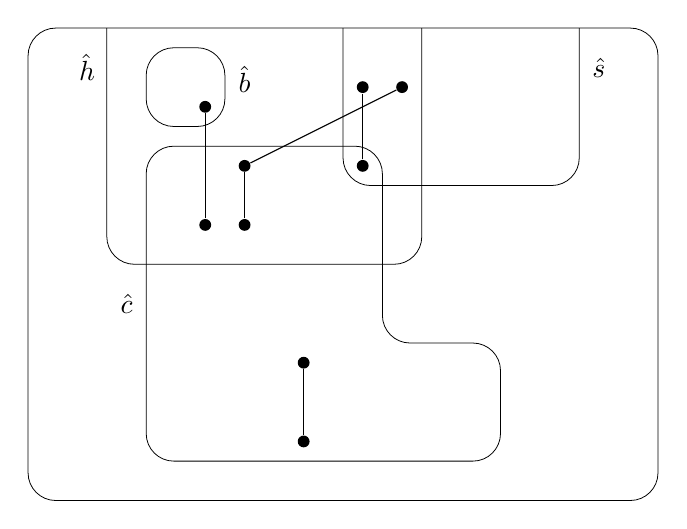
\begin{tikzpicture}[every node/.style={circle, fill=black, inner sep=0.5pt, minimum size=1.5mm}]
			]
			% \draw[help lines] (0,0) grid (8,6);
			\draw[rounded corners=10pt, line width=0.1mm] (0,0) rectangle (8,6);
			\draw[rounded corners=10pt, line width=0.1mm] (1,6) -- (1,3) -- (5,3) -- (5,6);
			\node[fill=none] (human) at (0.75,5.5) [] {$\hat{h}$};
			\draw[rounded corners=10pt, line width=0.1mm]
				(1.5,4.5) --
				(4.5,4.5) --
				(4.5,2) --
				(6,2) --
				(6,0.5) --
				(1.5,0.5) --
				cycle;
			\node[fill=none] (time) at (1.25,2.5) [] {$\hat{c}$};
			\draw[rounded corners=10pt, line width=0.1mm] (4,6) -- (4,4) -- (7,4) -- (7,6);
			\node[fill=none] (s) at (7.25, 5.5) [] {$\hat{s}$};

			\draw[rounded corners=10pt, line width=0.1mm] (1.5,5.75) rectangle (2.5,4.75);
			\node[fill=none] (billy) at (2.75,5.35) [] {$\hat{b}$};

			% minimal human
			% \draw[rounded corners=10pt, line width=0.2mm] (2,3) -- (2,4) -- (3,4) -- (3,3);
			% \node[fill=none] (minH) at (3.25,3.5) [] {$\underline{\hat{h}}$};
			\node (hb) at (2.25,3.5) [] {};
			\node (ht) at (2.25,5) [] {};
			\node (hr) at (2.75,3.5) [] {};
			\node (hrt) at (2.75,4.25) [] {};
			\draw (hr) -- (hrt);
			\draw (hb) -- (ht);

			% minimal soldier
			% \draw[rounded corners=10pt, line width=0.2mm] (5,5.25) -- (4.25,5.25) -- (4.25,4.25) -- (5,4.25);
			% \node[fill=none] (minS) at (5.25,5) [] {$\underline{\hat{s}}$};
			\node (sb) at (4.25, 4.25) [] {};
			\node (st) at (4.25, 5.25) [] {};
			\node (sr) at (4.75, 5.25) [] {};
			\draw (sb) -- (st);
			\draw (sr) -- (hrt);

			% minimal time
			% \draw[rounded corners=10pt, line width=0.2mm] (3,0.5) -- (3,1.25) -- (4,1.25) -- (4,0.5);
			% \node[fill=none] (minC) at (4.25,1) [] {$\underline{\hat{c}}$};
			\node (cb) at (3.5,0.75) [] {};
			\node (ct) at (3.5,1.75) [] {};
			\draw (cb) -- (ct);
		\end{tikzpicture}
		\caption{A preferential interpretation}
		\label{figure:preferential-interpretation}
	\end{figure}

	For the first observation, we remind the reader of \Cref{lemma:cut-cautious} which says that if $\phi \twiddle \psi$,
	then the plausible consequence of $\phi \land \psi$ coincide with those of $\phi$. Our interpretation is a model of $h
	\twiddle c$; moreover, the states included in $\underline{\hat{h}}$ are precisely those states given by $\underline{\widehat{h \land c}}$.

	\textcolor{red}{Second observation about why the semantics don't allow contraposition or transitivity, and maybe also monotonicity.}
\end{example}

Within the context of preferential models, there is another treatment of classical formulae which allows for the discarding
of \Cref{definition:state-satisfaction} and a single notion of what it means for a preferential interpretation to be a model
of a formula in $\Lang$. The idea is to translate the hard-constraints of classical formulae to defeasible counterparts,

\begin{lemma}
	\label{lemma:classical-to-defeasible} If $\phi$ is a classical formula in the language $\Lang$, then it can be
	expressed as the defeasible conditional $\neg \phi \twiddle \bot$. Then, any preferential interpretation $\pin$ is a
	model of $\phi$ if and only if it is a model of $\neg \phi \twiddle \bot$.
\end{lemma}

For $\pin$ to be a model of $\neg \phi \twiddle \bot$, it is equivalent to say that the minimal states which satisfy
$\neg \phi$ also satisfy $\bot$, or $\underline{\hat{(\neg \phi)}}\subseteq \hat{(\bot)}$. Of course, $\bot$ represents falsehood,
and the set of states which satisfy falsehood is the emptyset. In turn, there can be no states which satisfy $\neg \phi$,
equivalent to the condition that all states satisfy $\phi$. If $\phi$ is thought of as the proposition \say{All men are mortal},
then the defeasible counterpart reads as \say{If not all men are mortal, then it is normal to infer anything, including a contradiction}
\cite{kraus1990nonmonotonic,lehmann1992what}.

We assume this treatment of classical formulae from this point onwards, and consolidate the notation as
$\pin \VDash \phi$ where $\phi \in \Lang$ is a defeasible conditional.

\textcolor{red}{maybe something about how without smoothness, we don't have CM}

\begin{theorem}[Soundness]
	\label{theorem:soundness-preferential}

	If $\Pin$ is a preferential interpretation and $\phi, \psi \in \Lang$, then $\pin$ defines the consequence relation $\twiddle
	_{\pin}$ given by the set $\{\phi \twiddle_{\pin}\psi \mid \pin \VDash \phi \twiddle \psi\}$, which satisfies \textit{Reflexivity},
	\textit{Left Logical Equivalence}, \textit{Right Weakening}, \textit{Or}, and \textit{Cautious Monotony} and is thus a
	preferential consequence relation.
\end{theorem}

\begin{theorem}[Completeness]
	\label{theorem:completeness-preferential}

	If $\twiddle_{P}$ is a preferential consequence relation, then there exists a preferential interpretation $W$ which induces
	the consequence relation $\twiddle_{W}$ such that $\twiddle_{P}$ is precisely $\twiddle_{W}$.
\end{theorem}

The decision to construct a preference relation on states rather than valuations directly, and then map states to valuations,
may seem arbitrary. Certainly, Shoham \cite{shohamSemanticApproach} makes no such distinction in his preferential logic.
However, Kraus, Lehmann, and Magidor \cite{kraus1990nonmonotonic} provide an example of a preferential consequence
relation generated by a preferential model with a non-injective function mapping states to valuations which has no
injective counterpart which induces an equivalent consequence relation; the argument was aptly called \textit{en pessant}
in \cite{Bezzazi1997}.

Consider the more finely grained portion of the preferential interpretation in \Cref{figure:preferential-interpretation}.
As before, the interpretation is a model of the conditional $s \twiddle h$. It is not, however, a model of $s \twiddle c$
given that $s_{2}$, a duplicate state to $s_{1}$, is a minimal state satisfying $s$ which does not satisfy $c$.

\begin{figure}[H]
	\centering
	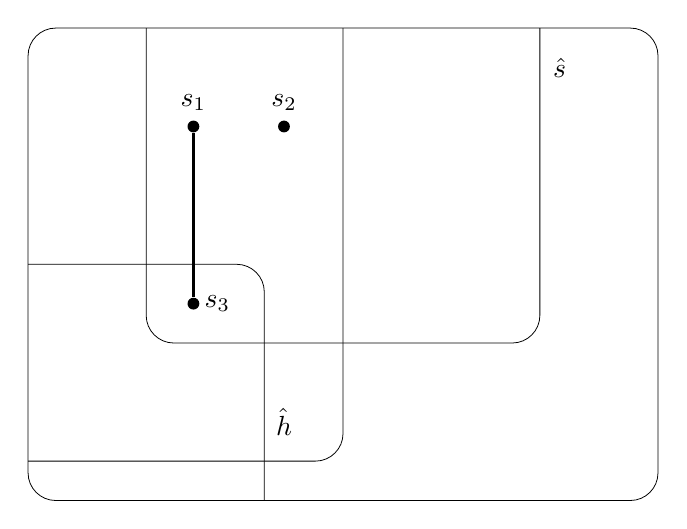
\begin{tikzpicture}[every node/.style={circle, fill=black, inner sep=0.5pt, minimum size=1.5mm}]
		% \draw[help lines] (0,0) grid (8,6);
		\draw[rounded corners=10pt, line width=0.1mm] (0,0) rectangle (8,6);
		\draw[rounded corners=10pt, line width=0.1mm] (1.5, 6) -- (1.5,2) -- (6.5,2) -- (6.5,6);
		\draw[rounded corners=10pt, line width=0.1mm] (4,6) -- (4,0.5) -- (0,0.5);
		\draw[rounded corners=10pt, line width=0.1mm] (0,3) -- (3,3) -- (3,0);

		\node[fill=none] (h) at (3.25, 1) [] {$\hat{h}$};
		\node[fill=none] (s) at (6.75, 5.5) [] {$\hat{s}$};

		\node (1) at (2.1,4.75) [label=above:{$s_{1}$}] {};
		\node (2) at (3.25,4.75) [label=above:{$s_{2}$}] {};
		\node (3) at (2.1,2.5) [label=right:{$s_{3}$}] {};
		\draw[line width=0.3mm] (1) -- (3);
	\end{tikzpicture}
\end{figure}

\subsection{Rational Consequence Relations}
\label{subseciton:rational-consequence-relations}

We now discuss a subset of preferential consequence relations which satisfy the additional property of \textit{rational
monotony}.

\begin{align}
	\inferLeft{Rational Monotony}{\phi \twiddle \psi, \quad \phi \ntwiddle \neg \gamma}{\phi \land \gamma \twiddle \psi}
\end{align}

The pattern of reasoning described by rational monotony is perhaps the most controversial of the KLM postulates. From
the perspective of knowing $\phi$ it is normal to conclude that $\psi$, but it is not necessarily normal to conclude $\neg
\gamma$---this latter clause is not saying it is normal to conclude $\gamma$. Rational monotony requires that should we
then move to a scenario where $\phi$ and $\gamma$ hold, all the inferences that were plausible when we knew only that $\phi$
held should remain.

Consider the following example of a university where it is normal (\textit{expected, typical}) for students to graduate.
Alice is a normal student and so she will graduate, but is also widely regarded as being quite a clever student. Bob is another
student who, despite being clever, is known by his professors to be unprecedentedly lazy. As a result of failing to
appear for his final examinations, Bob will not graduate.

Rational monotony would require that normal students who are also clever will graduate, and so there should always be a
clever student who is explicitly preferred (in the preference relation) to Bob. Preferential interpretations do not commit
us to this idea,

\begin{figure}[H]
	\centering
	\begin{minipage}{0.49\textwidth}
		\centering
		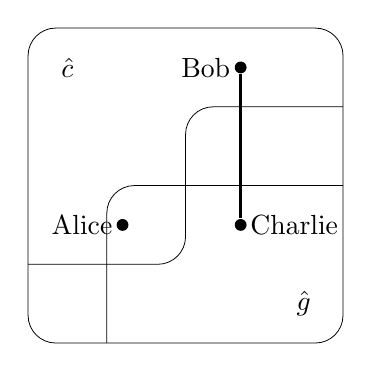
\begin{tikzpicture}[every node/.style={circle, fill=black, inner sep=0.5pt, minimum size=1.5mm}]
			% \draw[help lines] (0,0) grid (6,6);
			\draw[rounded corners=10pt, line width=0.1mm] (0,0) rectangle (4,4);
			\draw[rounded corners=10pt, line width=0.1mm] (0,1) -- (2,1) -- (2,3) -- (4,3);
			\draw[rounded corners=10pt, line width=0.1mm] (1,0) -- (1,2) -- (4,2);

			\node[fill=none] (clever) at (0.5,3.5) [] {$\hat{c}$};
			\node[fill=none] (graduated) at (3.5,0.5) [] {$\hat{g}$};

			\node (bob) at (2.7,3.5) [label=left:{Bob}] {};
			\node (charlie) at (2.7,1.5) [label=right:{Charlie}] {};
			\draw[line width=0.3mm] (bob) -- (charlie);
			\node (alice) at (1.2,1.5) [label=left:{Alice}] {};
		\end{tikzpicture}
		\subcaption{} \label{subfigure:not-rational}
	\end{minipage}
	\begin{minipage}{0.49\textwidth}
		\centering
		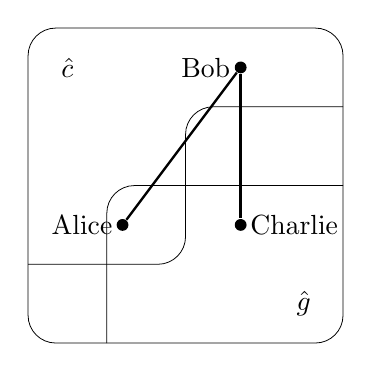
\begin{tikzpicture}[every node/.style={circle, fill=black, inner sep=0.5pt, minimum size=1.5mm}]
			\draw[rounded corners=10pt, line width=0.1mm] (0,0) rectangle (4,4);
			\draw[rounded corners=10pt, line width=0.1mm] (0,1) -- (2,1) -- (2,3) -- (4,3);
			\draw[rounded corners=10pt, line width=0.1mm] (1,0) -- (1,2) -- (4,2);

			\node[fill=none] (clever) at (0.5,3.5) [] {$\hat{c}$};
			\node[fill=none] (graduated) at (3.5,0.5) [] {$\hat{g}$};

			\node (bob) at (2.7,3.5) [label=left:{Bob}] {};
			\node (charlie) at (2.7,1.5) [label=right:{Charlie}] {};
			\draw[line width=0.3mm] (bob) -- (charlie);
			\node (alice) at (1.2,1.5) [label=left:{Alice}] {};
			\draw[line width=0.3mm] (bob) -- (alice);
		\end{tikzpicture}
		\subcaption{} \label{subfigure:rational}
	\end{minipage}
	\caption{ Two preferential models of the above scenario; \textit{sub-figure a} does not satisfy rational monotony,
	while \textit{b} does.}
\end{figure}

It is quite easy to spot the culprit: The preference relation does not impose strong enough restrictions on how incomparable
objects should be treated.

\begin{definition}
	\label{definition:modular-order} \index{partial-order! modular}

	A partial order $\prec$ on the set $X$ is \emph{modular} if and only if for any incomparable $x,y \in X$ when $z \prec
	x$ then also $z \prec y$.
\end{definition}

Under a modular partial order, incomparability can be considered an equivalence relation on the respective set where incomparable
elements fall into equivalence classes \cite{GinsberCounterfactuals,lehmann1992what}. We now introduce \textit{ranked
interpretations} as a structure which assigns to each of these equivalence classes a rank describing the preference relation
on worlds.

\begin{definition}
	\label{definition:ranked-interpretation}

	A \emph{ranked interpretation} is a preferential interpretation $\Pin$ where the preference relation $\prec$ is \emph{modular}.
\end{definition}

One consequence, in terms of the way they are represented, is that ranked interpretations can be visualised as a
stratification of states, rather than Hasse diagrams. The preferential interpretation in \Cref{subfigure:rational}, which
has a modular preference relation and can accordingly be considered a ranked interpretation, can be visualised as the
following structure:

\begin{figure}[H]
	\centering
	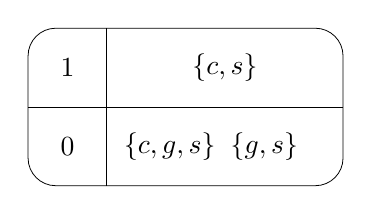
\begin{tikzpicture}[every node/.style={circle, fill=black, inner sep=0.5pt, minimum size=1.5mm}]
		\draw[rounded corners=10pt, line width=0.1mm] (0,2) rectangle (4,0);
		\draw[rounded corners=10pt, line width=0.1mm] (0,1) -- (4,1);
		\node[fill=none] (0) at (0.5,0.5) [] {$0$};
		\node[fill=none] (1) at (0.5,1.5) [] {$1$};
		\draw (1,0) -- (1,2);
		\node[fill=none] (alice) at (1.8,0.5) [] {$\{c,g,s\}$};
		\node[fill=none] (charlie) at (3,0.5) [] {$\{g,s\}$};
		\node[fill=none] (bob) at (2.5,1.5) [] {$\{c,s\}$};
	\end{tikzpicture}
	\caption{A depiction of a ranked interpretation}
\end{figure}

\begin{lemma}
	\label{lemma:modular-ranking-function}

	If $\prec$ is a modular partial order on $X$ then there is a \emph{ranking function} $\mathsf{r}\colon X \to \Omega$,
	with $\Omega$ being a totally ordered set for which the strict order is denoted $<$, such that if $x \prec y$ then $\mathsf{r}
	(x) < \mathsf{r}(y)$ for any $x,y \in X$.
\end{lemma}

The

\clearpage
The reasoning pattern described by rational monotony is the most controversial of the KLM postulates We can understand rational
monotony as describing a pattern of reasoning where, under normal circumstances, the presence of $\phi$ means the presence
of $\psi$ and not necessarily the presence of $\neg \gamma$ (there is at least one normal $\phi$-states where $\gamma$
holds). Then, assuming that $\gamma$ does indeed hold should not result in the withdrawal of any plausible inferences that
were made from $\phi$.

The question that requires consideration is whether, from this description, it should be possible for Bob to be considered
as a typical, clever student; or, must we concretely hold the view that Alice is a more typical clever student than Bob?
A preferential interpretation does not commit us to either view, we show below two preferential interpretations
entertaining both perspectives

\textcolor{red}{Smoothness is always satisfied by ranked models with a finite language}

\begin{definition}
	\label{definition:rational-consequence-relation} \index{consequence relations! rational}

	The consequence relation $\twiddle_{R}$ is a \emph{rational consequence relation} if and only if it satisfies \textit{Reflexivity},
	\textit{Left Logical Equivalence}, \textit{Right Weakening}, \textit{Cut}, \textit{Cumulative Monotony}, and \textit{Rational
	Monotony}.
\end{definition}

Rational consequence relations quite clearly satisfy all the conditions of preferential consequence relations. The reason
that certain preferential interpretations fail to satisfy rational monotony is due to what is permitted in their preference
relations. \Cref{subfigure:not-rational} is a model of $s \twiddle g$, and it does not satisfy $s \twiddle \neg c$.

Because of the need for states, we have this defect which prevents rational monotonicity from being satisfied. If we really
want rational monotony, we have to have a modular order.

\subsection{Preferential Entailment}

RE iT not being nmr We are willing to accept these credulous inferences precisely because they may be retracted we may withdraw
previous inferences under learning new facts.

\section{Rational Closure}

\subsection{Rational Consequence Relations}